\documentclass[11pt, a4paper, oneside]{article}
\setlength{\parindent}{0pt}
\newlength{\drop}
\usepackage{textcomp}
\usepackage{float}
\usepackage{caption}
\usepackage{subcaption}
\usepackage{graphicx}
\usepackage{fancyhdr} % For headers and footers
\usepackage{vhistory} % For revision history
\usepackage{enumerate}
\usepackage{hyperref}
\hypersetup{
    colorlinks,
    citecolor=black,
    filecolor=black,
    linkcolor=black,
    urlcolor=black
}

\pagestyle{fancy}
\lhead{EV3 Test Report}
\rhead{\thepage}
\cfoot{}

\begin{document}
  \begin{titlepage}
    \drop=0.1\textheight
    \centering
    \vspace*{\baselineskip}
    \rule{\textwidth}{1.6pt}\vspace*{-\baselineskip}\vspace*{2pt}
    \rule{\textwidth}{0.4pt}\\[\baselineskip]
    {\scshape \LARGE Test report \\[0.3\baselineskip] for EV3 Robot Kit}\\[0.2\baselineskip]
    \rule{\textwidth}{0.4pt}\vspace*{-\baselineskip}\vspace{3.2pt}
    \rule{\textwidth}{1.6pt}\\[\baselineskip]
    {\scshape Issued for:  University of Adelaide}\\[0.2\baselineskip]
    \vfill
    \scshape
    Authors: \\ Xiang Guo (a1077337) \\ Thomas McAtee (a1608768) \par
    \vspace*{2\baselineskip}

    {\large December 19th 2014}\par
      \thispagestyle{empty}

  	\end{titlepage}

  \thispagestyle{empty}
  \newpage


  \tableofcontents
  \thispagestyle{empty}
  \newpage
  \setcounter{page}{1}
  	\section{Introduction}
	This report was created to test the functionality of the new Lego EV3 Robot kit acquired by the University of Adelaide for potential use as part of future Software Engineering Project course. The EV3 will be tested against the previously used Lego NXT Robot kits and judged on their feasibility to replace the older NXT Robot.\\

	The following sections will provide a brief overview on some of the differences between the NXT and the EV3. For more details please refer to the rest of this document.

		\subsection{Brick Comparison}


		\begin{figure}[H]
		\begin{subfigure}{.45\textwidth}
		  \centering
		  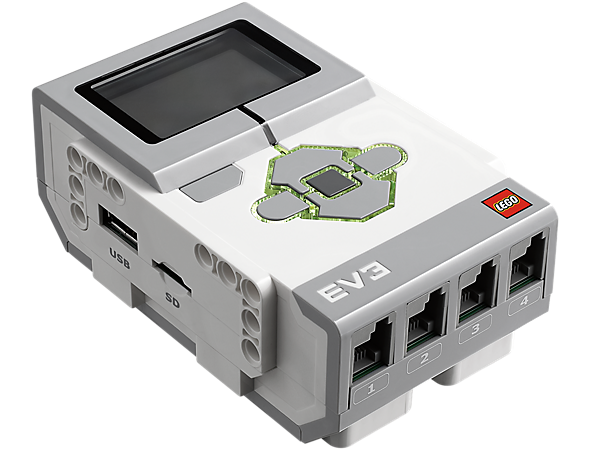
\includegraphics[scale=0.23]{img/EV3Brick.png}
		  \caption{EV3 Brick}
		\end{subfigure}%
		\begin{subfigure}{.45\textwidth}
		  \centering
		  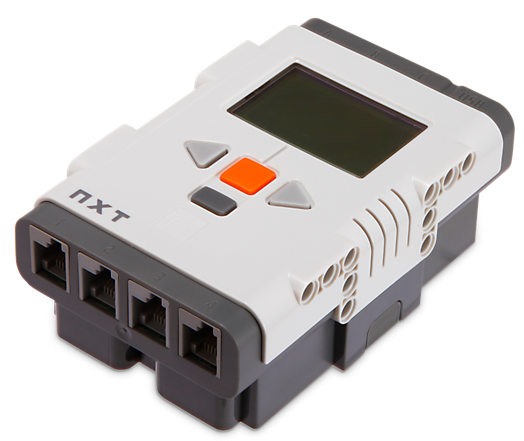
\includegraphics[scale=0.35]{img/NXTBrick.png}
		  \caption{NXT Brick}
		\end{subfigure}
		\end{figure}
	



		\subsection{New Features}
		
		\begin{figure}[H]
	  	\centering
	  	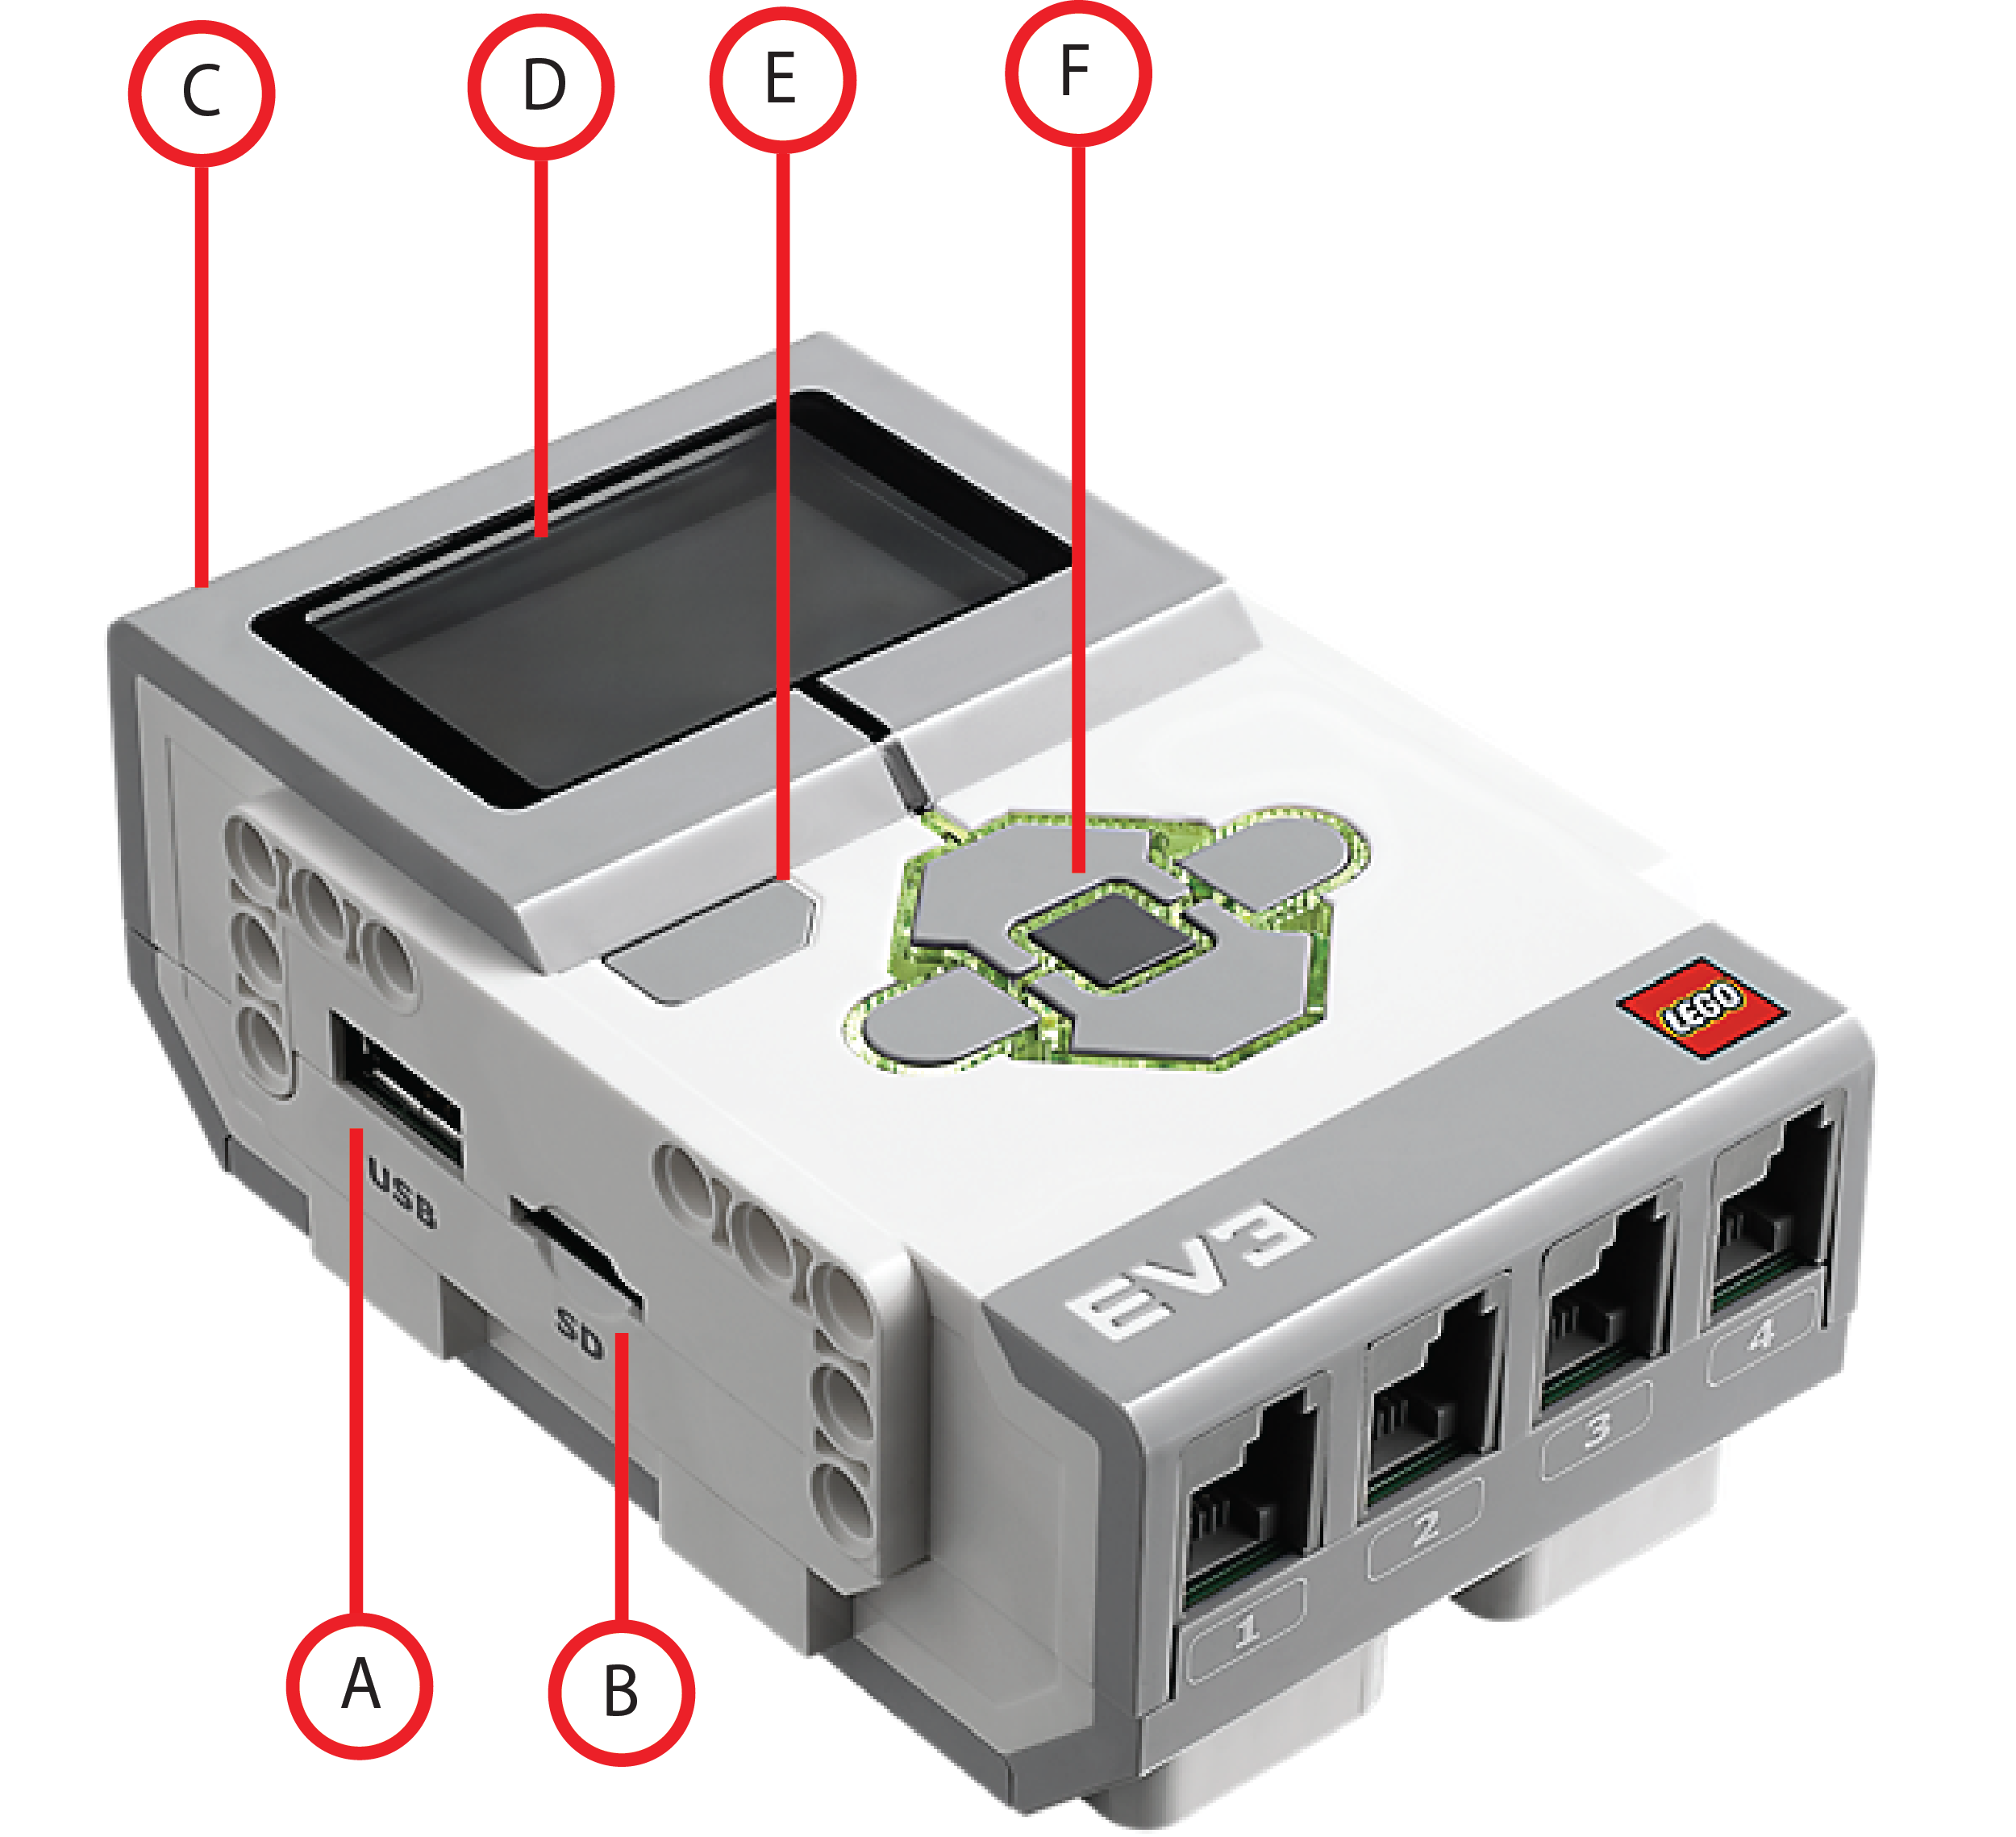
\includegraphics[scale=0.45]{img/EV3Brick_Labelled.png}
		\caption{EV3 Brick with new features}
		\end{figure}

		\begin{enumerate}[A:]
		\item USB Host Port - Can be used currently to connect WiFi dongle. Other hardware are possible such as keyboard, mouse, USB Memory stick, web cam etc but subject to availability of additional software.
		
		\item Micro SD card slot - Can support up to 32 gb SD cards as long as it is Fat-32.
		
		\item Motor Ports - 4 ports in total, 1 more than the NXT Brick.
		
		\item LCD Screen - More than double the pixel resolution of the NXT brick.
		
		\item Shifted button - Exit/Cancel button location shifted.
		
		\item Additional buttons - 2 additional buttons compared to the NXT Brick, there are Up and Down respectively.
		
		\end{enumerate}
		
		
	

		

 		\subsection{Improvements}
 		\begin{itemize}
 		\item EV3 Bump sensor is slightly shorter than the NXT Bump Sensor.
 		\item EV3 Ultrasonic sensor is slightly longer than the NXT Ultrasonic Sensor, but is vastly improved.
 		\item EV3 Colour sensor is much improved compared both the NXT colour and light sensor.
 		\item EV3 Pivot wheel design is much improved.
 		\end{itemize}
 		

 		


		
 		
 		
 		
 		
 		
 		
	\section{Hardware}
	\subsection{EV3 Brick}
		\subsubsection{Display}
		\begin{itemize}
			\item Resolution more than tripled. EV3:178x128 (Total pixels: 22784) vs NXT: 100x64 (Total pixels:6400).
			\item Improved exception feedback. NXT exception feedback came in the form of a code which needs to be checked against a table. EV3 screen displays a full non-wrapping stack trace which is navigable using the hardware buttons.
			\item Coordinates on screen has changed. 0,0 on NXT was the bottom left of screen. 0,0 is top left on EV3 display.
		\end{itemize}
		
		\subsubsection{Ports}
		\begin{itemize}
			\item Modified RJ-12 connector: The EV3 still uses the same type of proprietary  modified RJ-12 connector that NXT used. These differ from normal RJ-12 connectors and the position clip is located off-centre. These connectors can be purchased online if needed.
			\item 5 sensors supplied with the kit but only 4 sensor ports available. There are after market hardware which will allow multiple sensors to be attached to one port. But this requires heavy amount of permanent modifications to the sensor cables which is not advised.
			\item USB port can be used to connect up to 4 EV3 bricks which allows for control of up to 16 motors and 16 sensors on one robot.
			\item USB port can be used with a WiFI dongle to provide WiFi connectivity(see section 4 for more details.)
			\item USB port can be used to connect a wide range of accessories such as keyboard, mouse, web cam etc. This is subject to availability of software drivers for the device.
			\item Micro SD port supports up to a 32gb SD card. Can be used to increase brick storage, but mainly as the boot drive for LeJOS. SD card needs to be formatted using FAT32.
		
		\end{itemize}
		
		\subsubsection{Connections}
		\begin{itemize}
			\item Bluetooth connectivity
			\item USB connectivity (both via mini USB and via a USB host port). The host port also supports slave EV3 devices.
			\item Wireless connectivity; the device has support for a USB wifi dongle
		\end{itemize}
		\subsubsection{Battery}
		\begin{itemize}
			\item Lithium ion (AA battery pack also supplied)
			\item 2050mAh compared to 2100mAh of the NXT.
			\item The EV3 seems to have better battery performance than the NXT battery that was tested. This was most likely due to the age of the NXT kits.
		\end{itemize}
		\subsubsection{Buttons}
The EV3 button interface has greatly improved over the NXTs by the simple addition of two extra buttons to make six buttons. This allows two dimensional navigation rather than single dimensional navigation (as there are now four directional buttons rather than just two) and has a very handy backlight for button visibility in dark areas.\\
The new button scheme can be observed in figure 2.

  	\subsection{Sensors}
  		\subsubsection{Light}
		
  		The same module as the NXT Robot. New API on EV3 which returns a float instead of an int. Accurate to 2 decimal places. New API does not allow calibration (which isn't a new feature; the NXT API did not include methods to truly calibrate the sensor anyway, it simply created upper or lower bounds and normalised the returned data). If users wish to do this kind of soft calibration, they can use the source code for the NXT LeJOS API as a guide. \\

  		Has two modes, reflection and ambient. Reflection is the default mode and should be used for line following code. Black lines on normal print paper show up at around 40\% reflection whereas white paper shows up as roughly 75\%.

  		Ambient mode can be used to detect light sources. This could potentially be used to orientate a robot based on a nearby light source.

  		\subsubsection{Color}
		\begin{figure}[h]
		\centering
		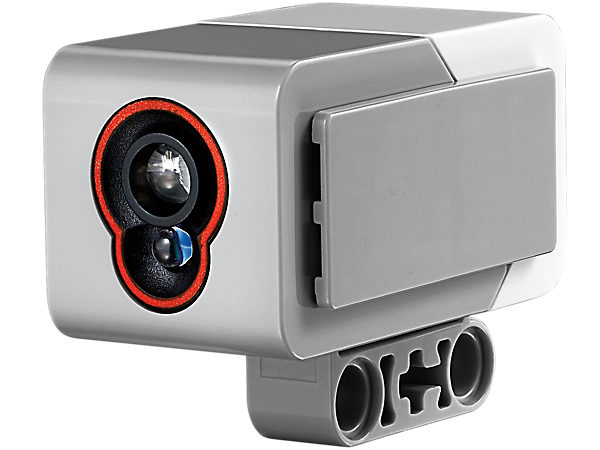
\includegraphics[scale=0.45]{img/EV3ColorSensor.png}
		\caption{EV3 Color Sensor}
		\end{figure}
  		The Color sensor has three modes: Reflection, Ambient and Color. Ambient and Reflection modes are the same as the Light Sensor equivalent, however the sensitivity of the sensor while measuring both is different. \\

  		Ambient mode is around half the sensitivity of the Light Sensor which means it should be able to differentiate between relatively bright light sources but might have trouble differentiating low level light sources. \\

  		Reflection mode is much more sensitive than the Light Sensor. Black lines on standard paper at 10mm range returned a reflection result of around 10 percent whereas white paper at the same distance returned 70 to 80 percent. This increased sensitivity should help in the project for Line Following and should be able to better handle smudges and imperfections on the test maps if the user implements a suitable tolerance in the code. \\

  		The color mode is meant to differentiate between up to 8 different colors, black, gray, red, green, yellow, blue, magenta, white. Testing was done using a laser printed standard 80gsm A3 paper, which contained a 256 color RGB chart. All tests were conducted at a range of approximately 5mm and at varying angles between 60 to 120 degrees. The sensor was able to pick up solid primary�� colors without issue at the angles tested. By primary we mean any colour where it's RGB hex value was represented by only pairs of F or 0. Eg. FFFFFF for white, FF0000 for red, FFFF00 for yellow etc. \\

  		Intermediate colors produced mixed results depending on the angle. Eg. FF8700 can be recognised as red at certain angles and as yellow at other angles. This is due to the reflection of the floodlight used by the sensor and the reflectivity of the ink on the paper. Therefore it is recommended in future projects to use only primary� colors and non reflective paper to reduce the likelihood of erroneous readings. Other precautions that can be taken is to use colors that a true primary RGB e.g. Black 000000, white, FFFFFF, Red FF0000, Green 00FF00 or Blue 0000FF only and calibrate the sensor to only return one of those options. \\



		\subsubsection{Gyroscope}
		This new sensor is amazing when actually working. It will report either changes to the angle, or rate of change to the angle of the sensor with a decent amount of accuracy (plus or minus a degree or two). \\
		
		\begin{figure}[H]
		\centering
		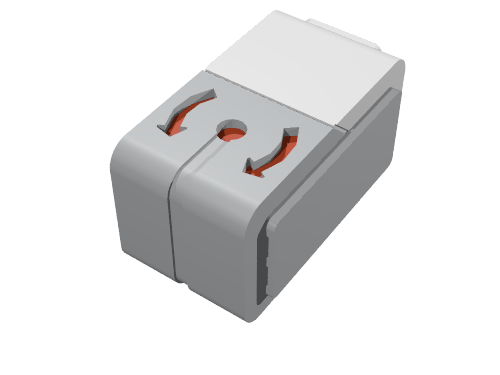
\includegraphics[scale=0.45]{img/EV3GyroSensor.png}
		\caption{EV3 Gyroscope Sensor}
		\end{figure}
		

		During testing it was noted that an error that causes a sensor “drift” occasionally appears where the sensor reading will slowly increment or decrement. Using the Lego test suite, this issue could be solved by unplugging and replugging the sensor from the port. However, using the standard LeJOS test suite, unplugging the sensor resulted in an exception which it was not able to recover from even when sensor is replugged in. A restart of the brick may be required if this bug appears. This will be something of concern if future students wish to incorporate the sensor in a project. This appears to be a firmware issue, and not related to LeJOS, future firmware releases may address this issue. Please note that this bug will appear straight away when the sensor is activated, it will not occur mid operation. So if the sensor is properly started and checked when the brick is turned on, it should not present a problem later during other operations. It is then advised to have a gyroscope test in LeJOS before starting any main programs.\newline
		
		The gyroscope instantly decreases the complexity of some of the robots algorithm as it no longer relies on tachometer readings to calculate it's current angle. The old way of angle calculation was very much prone to error as any wheel spin will cause errors in the result. \newline 

		Using the rate of change mode, you can accurately detect how many degrees per second the gyroscope is moving. This can be used a number of different ways such as limiting the speed of rotation on an action etc.


  		\subsubsection{Ultrasonic}
		\begin{figure}[H]
	  	\centering
	  	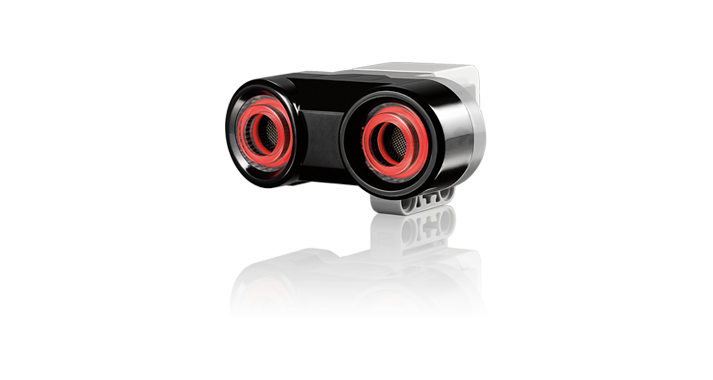
\includegraphics[scale=0.45]{img/EV3UltrasonicSensor.png}
	  	\caption{EV3 Ultrasonic Sensor}
		\end{figure}	 
		
		Much more accurate than the NXT sensor. Testing against different objects under 40cm distance against a tape measurer revealed a much improved sensor in the new kit. The EV3 US sensor had much higher fidelity and returned measurements in 1mm increments although the accuracy can have a margin of error between +- 4mm when detected surface was front on to the sensor. The older NXT US sensor was only able to report in 1cm increments and much higher margin of error of +- 3cm. \\

  		The minimum range of the sensor was also much improved. The NXT sensor loses accuracy within roughly 12cm. EV3 sensor was able to maintain accuracy to within 4cm. \\

  		The new sensor's cone of detection remains relatively narrow, no different to the NXT version. And both sensors suffer decreases in accuracy when the detected surface is at a sharp angle. The EV3 sensor was able to maintain accuracy when detected surface is at no more than 30 degree angle to the sensor(where 0 degree means completely front on to the sensor).\\


  		\subsubsection{Bump}
		\begin{figure}[H]
	  	\centering
	  	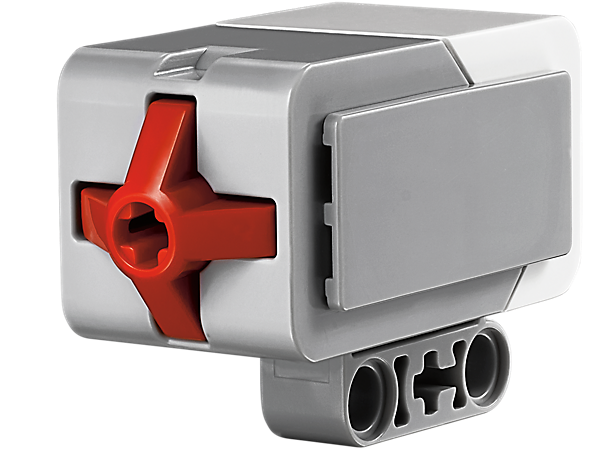
\includegraphics[scale=0.25]{img/EV3BumpSensor.png}
		\caption{EV3 Bump Sensor}
		\end{figure}	 		
 		
 		The EV3 bump sensor is physically shorter than the NXT equivalent. The EV3 sensor is 44mm while the NXT sensor is 48mm. They were identical in performance.  		
  		
  		
  		\subsubsection{Backwards Compatibility}
  		All NXT sensors can be used on the EV3 Brick with out issue. However, EV3 sensors will not be recognised by the NXT brick.

	\subsection{Motors}
		\subsubsection{Large}
		\begin{figure}[H]
	  	\centering
	  	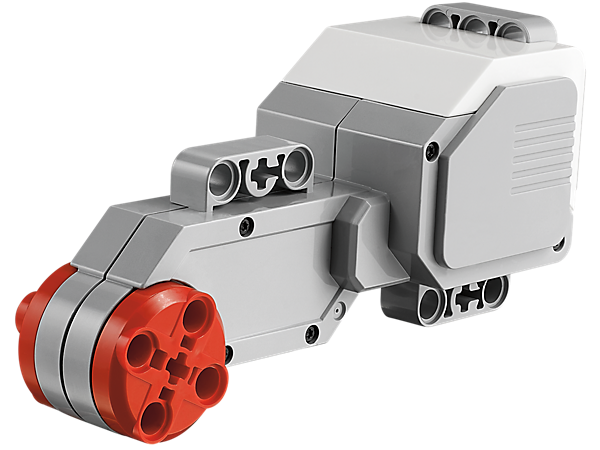
\includegraphics[scale=0.45]{img/EV3LargeMotor.png}
		\caption{EV3 Large Motor}
		\end{figure}		
		
		The EV3 large motor is comparable with the NXT regulated motor. In testing the NXT motor is slightly more efficient and achieved higher RPM accross multiple voltages compared to the EV3 motor. The differences are negligible when considering the scope of this project. 
		


		\subsubsection{Medium}
		The rotation sensor is a motor with less torque than a Large motor (typically used to move the robot) but with higher speed due to it's smaller diameter (it is capable of 260 RPM rather than the Large's 175). \\

		Possible problems: depending on the application it may be very important to keep track of the 'arm' being moved by the motors position. In tests it proved very easy to cause the shovel arm (design included in the Lego build manual) to collide with the motor itself which could potentially damage the internal mechanics of the motor.\\

		\begin{figure}[H]
	  	\centering
	  	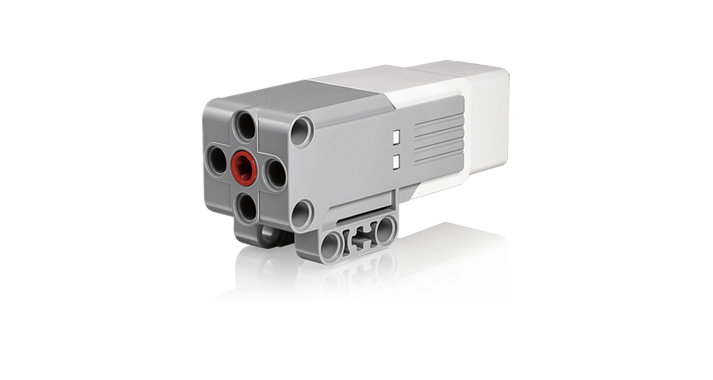
\includegraphics[scale=0.45]{img/EV3MediumMotor.png}
		\caption{EV3 Medium Motor}
		\end{figure}	
		
		(insert image of collision here)\\

		To counteract this, it may be necessary to 'reset' the position of the arm during device shutdown (this method description implies that the maintained 'position' of the motor will be reset upon a device reset)\\

		The Rotation Sensor utilises a motor port, which as part of the project shouldn't be a problem as students will only be provided with three modules that can utilise the four ports.

		\subsubsection{Backwards Compatibility}
		All NXT motors are compatible with the EV3 brick. EV3 motors can function with the NXT brick. In both cases use NXTRegulatedMotor class.
		
		\subsubsection{Enhancement}
		As noted on Wikipedia ( \url{https://en.wikipedia.org/wiki/Lego_Mindstorms_EV3#Enhancements}), the EV3 motors can be hacked to increase the resolution of the encoder. This required updating the firmware with a modified version. While there are significant benefits to this modification, it is most likely unnecessary for projects considered for this course. But having this option is a positive in favour of the EV3.		
		
	\subsection{Building blocks}
		\subsubsection{Pivot wheel}
		New ball bearing style pivot wheel design is excellent with omni directional movement. NXT pivot wheel design often resulted in uncontrolled shift in robot position when reversing or sharp turns. The new EV3 ball bearing wheel design completely solves this issue by allowing 360 degree movement without any mounting blocks moving. Still has issues when moving over edge of paper. Recommend sticky-taping test maps down to surface of table for any testing.
		
		\subsubsection{Frames}
		The addition of several pre-made rectangular frames greatly assists robot design and build. Many of the other pieces (such as the EV3 sensor modules) easily and logically slot in to varying positions on these frames to allow quick, intuitive and strong robot designs.
		
		\begin{figure}[H]
		\begin{subfigure}{.45\textwidth}
		  \centering
		  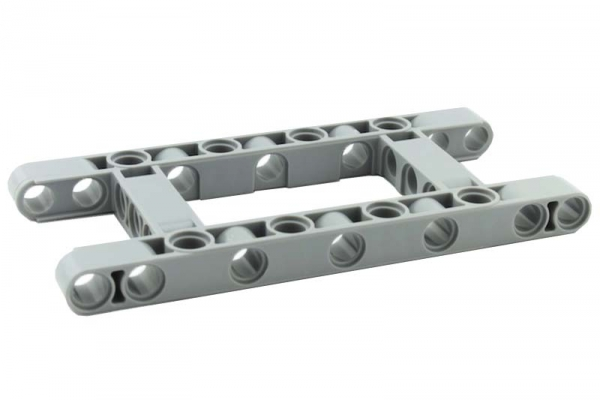
\includegraphics[scale=0.23]{img/Frame1.jpg}
		  \caption{Part 4540797}
		\end{subfigure}%
		\begin{subfigure}{.45\textwidth}
		  \centering
		  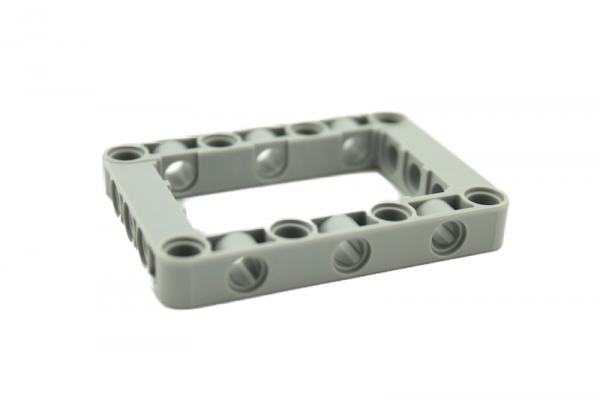
\includegraphics[scale=0.23]{img/Frame2.jpg}
		  \caption{Part 4539880}
		\end{subfigure}
		\end{figure}		
		
		\subsubsection{Sensor mounts}
		Every sensor now has an axle connector between two standard round holes. These axle connectors allow for quick mounting of any new sensor in essentially any desired position on the robot.
		\begin{figure}[H]
	  	\centering
	  	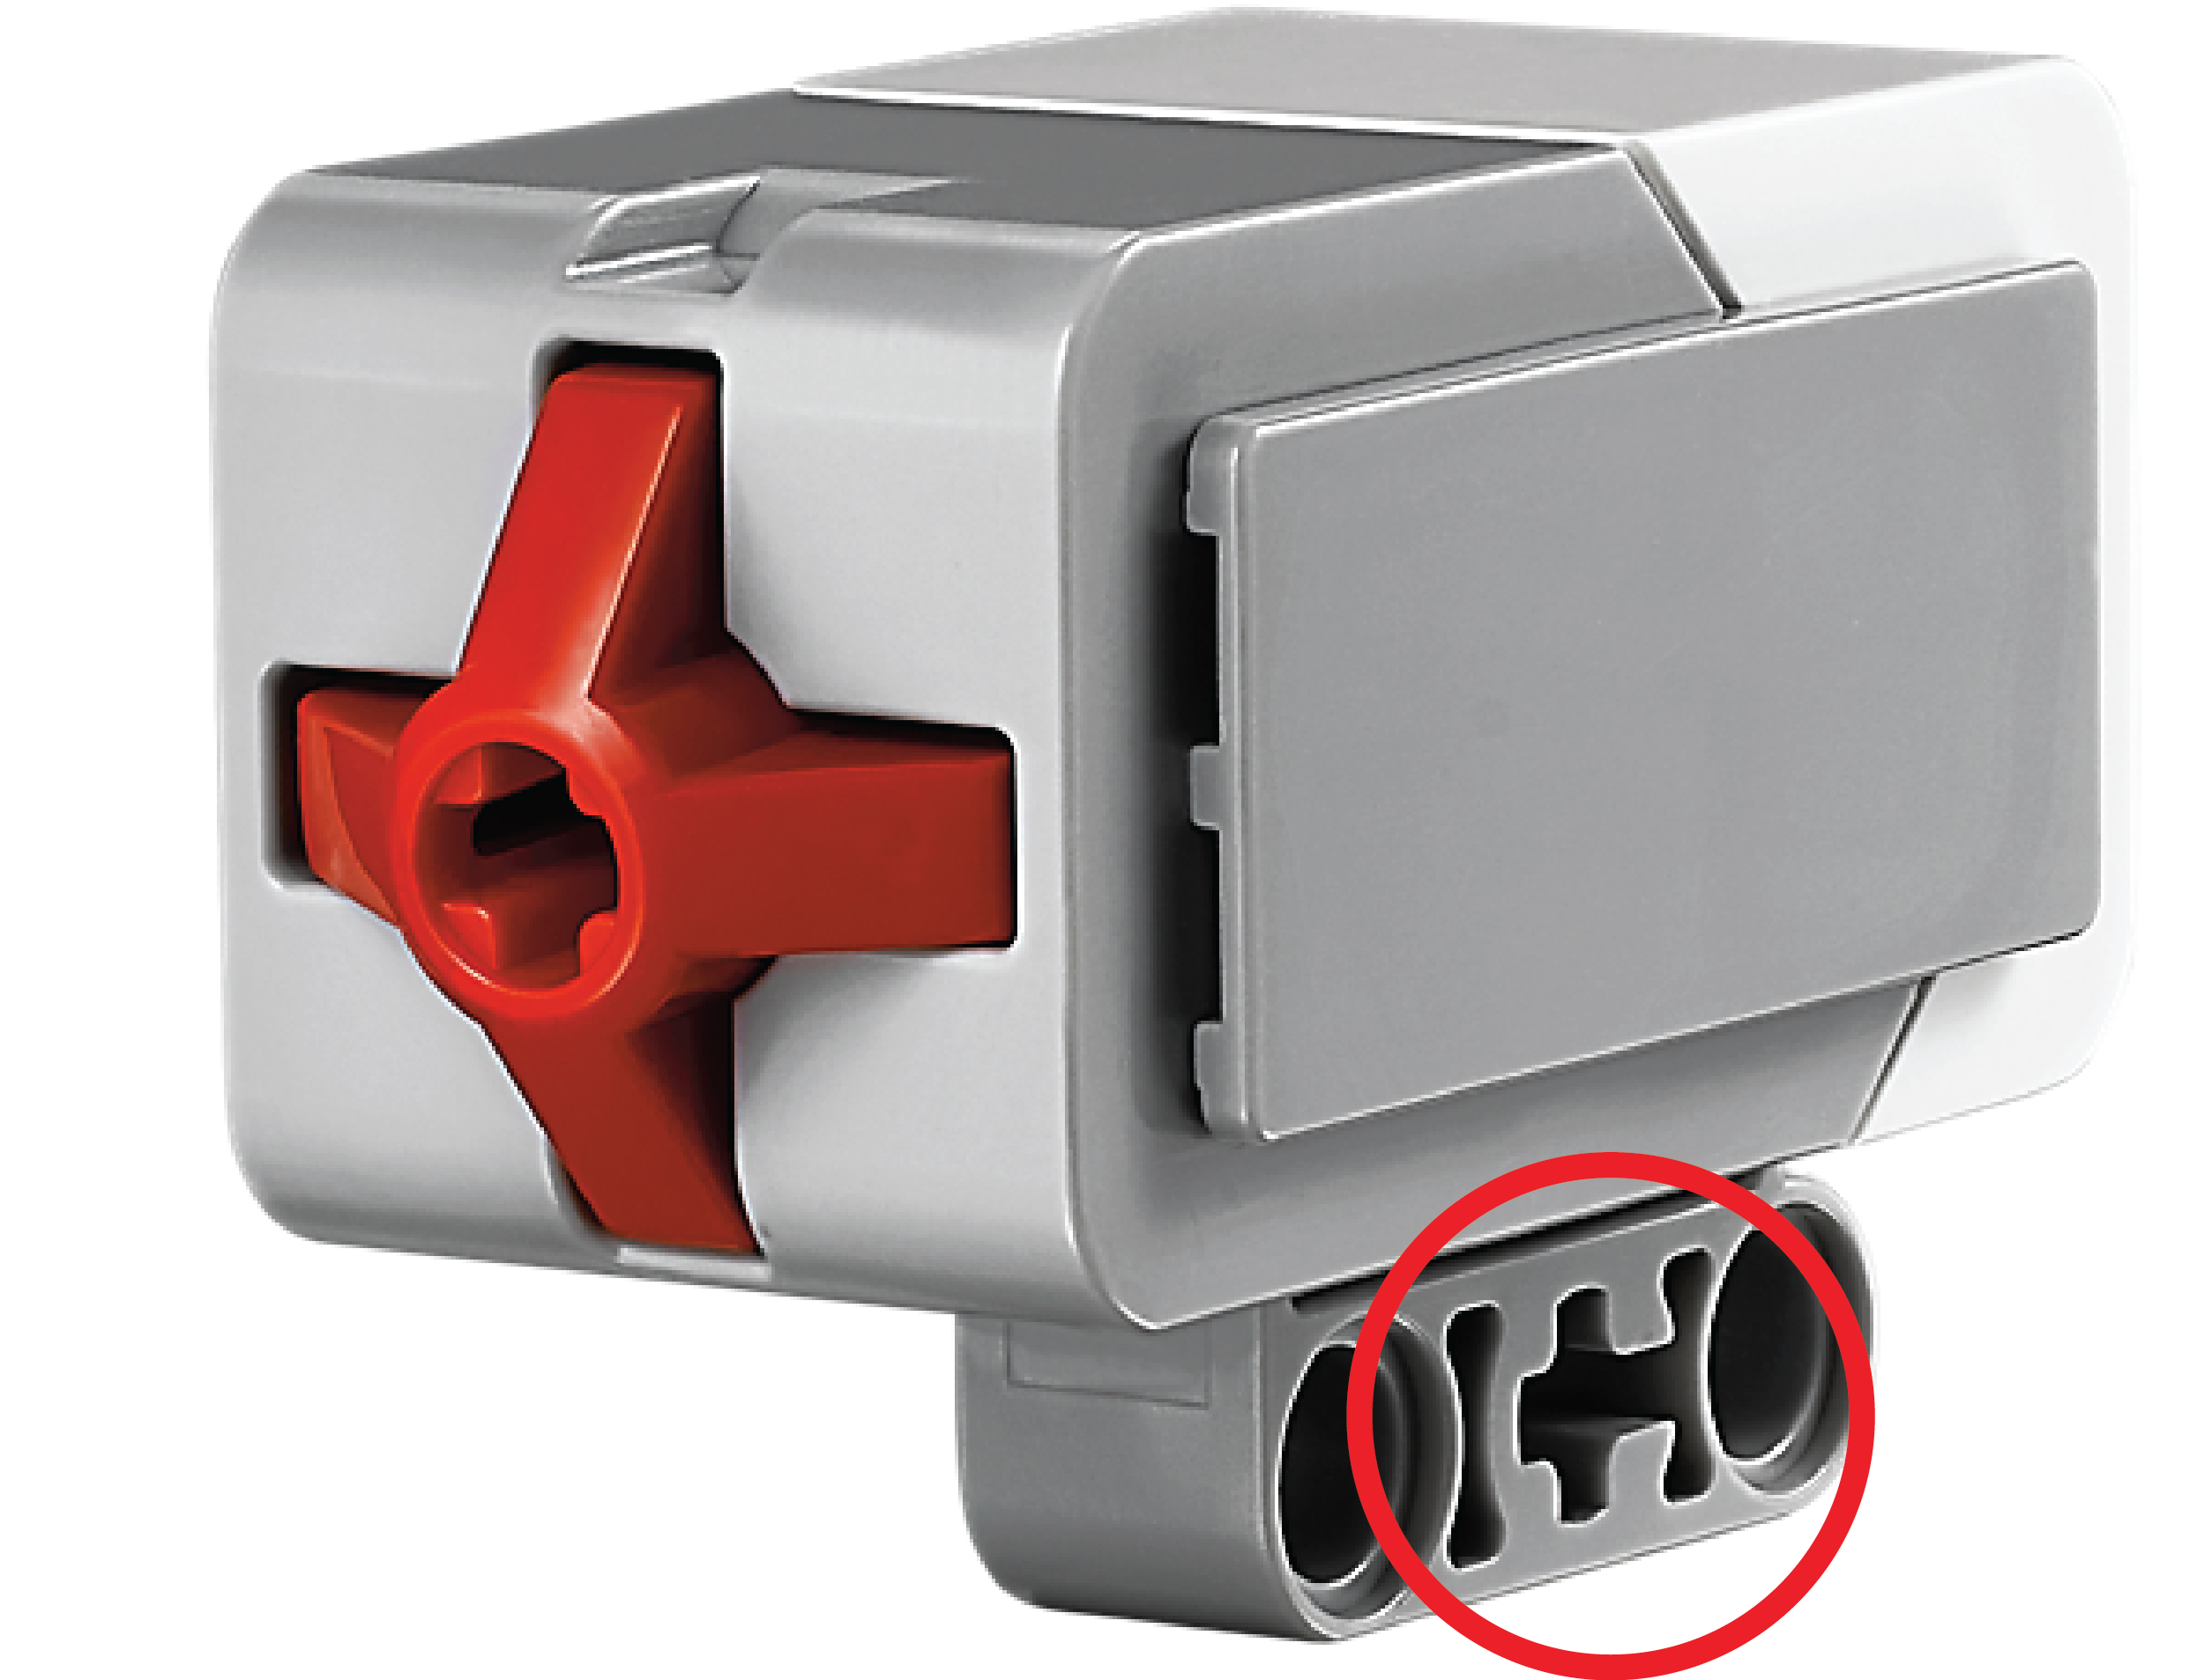
\includegraphics[scale=0.25]{img/EV3SensorMount.png}
		\caption{EV3 Sensor mount indicated by red circle.}
		\end{figure}			
		

	\section{Software}
	\subsection{Eclipse}
	Each version of leJOS has been released alongside plugins for Eclipse which enabled a high level of integration between the leJOS library and the Eclipse IDE. The NXT block allowed for relatively simplistic functionality however the EV3 plugin is quite improved and allows for advanced functionality such as:
	\begin{itemize}
		\item The ability to push code straight to the EV3 brick with minimal configuration (almost none is required if a USB connection is utilised).\\ 
		\item Fully leJOS API documentation; meaning to see what a method does it's only necessary to hover over the method signature with the mouse (rather than investigating it in an internet browser window).
		
	\end{itemize} 
	
	\subsubsection{Installation}
		\begin{enumerate}
		\item Make sure you have installed Java JDK and the leJOS software from this site \url{http://www.lejos.org/ev3.php}
		
		\item Start Eclipse
		
		\item Go to Help then Install New Software on the top menu bar(see Figure 10)
		
		\begin{figure}[H]
	  	\centering
	  	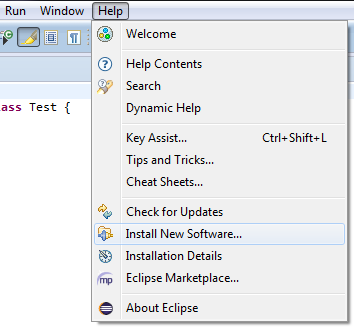
\includegraphics[scale=0.95]{img/Eclipse01.png}
	  	\caption{ }
		\end{figure}	
				
		\item An Install window will pop up. Click the Add button in the top right corner of the window.
		
		\item Give the respository a name such as "EV3 LeJOS". Then enter the URL \url{http://lejos.sourceforge.net/tools/eclipse/plugin/ev3} in the Location test box and click OK.(see Figure 11)
		
		\begin{figure}[H]
	  	\centering
	  	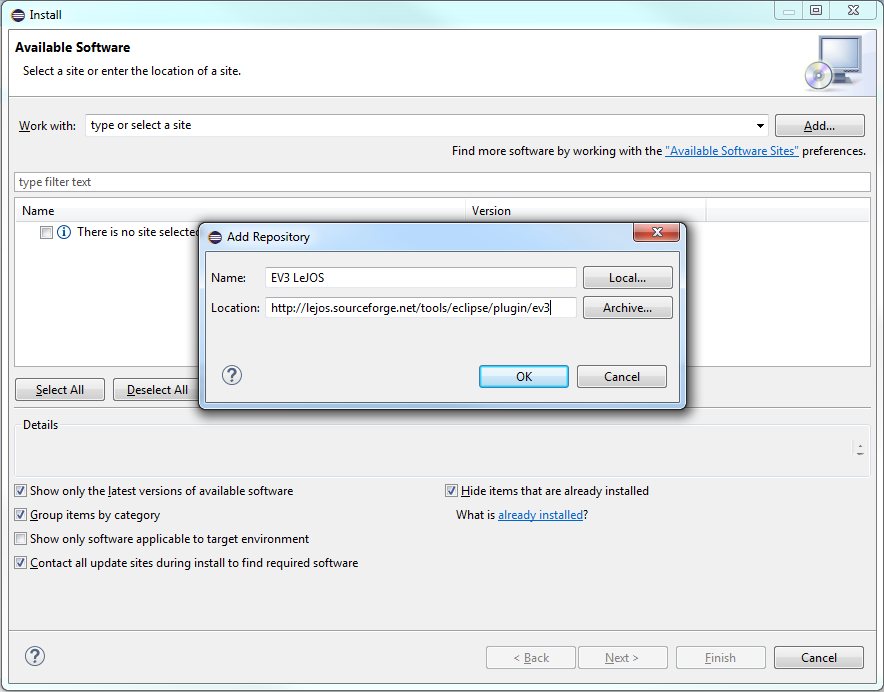
\includegraphics[scale=0.55]{img/Eclipse02.png}
	  	\caption{ }
		\end{figure}
		
		\item In a few seconds "leJOS EV3 Support" will appear in the selection box. Check the tick box next to this and click Next. Eclpse will now calculate the requirements and dependencies for the plugin, this step can take a minute or so. (see Figure 12)
		\begin{figure}[H]
	  	\centering
	  	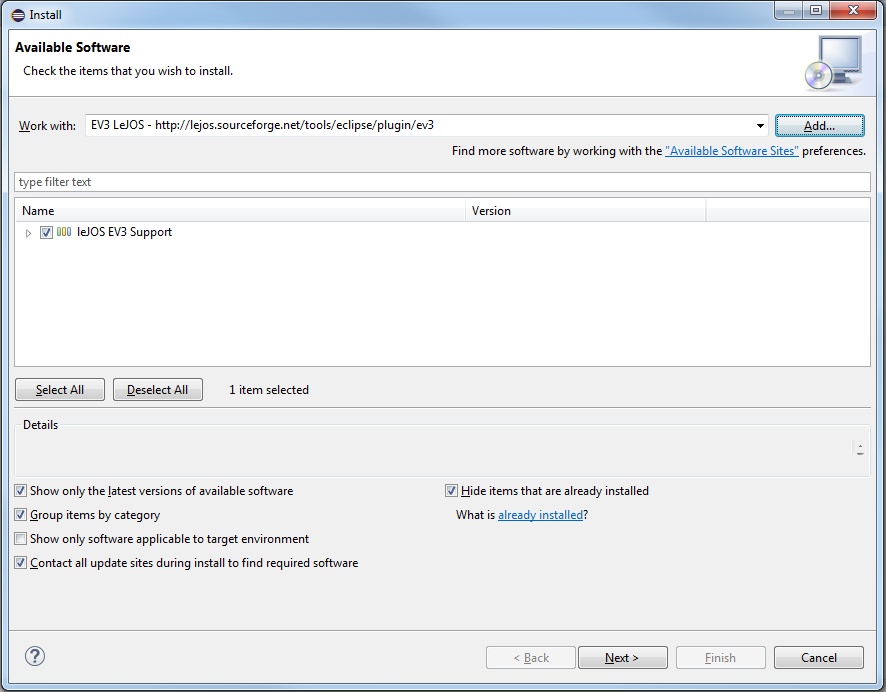
\includegraphics[scale=0.55]{img/Eclipse03.png}
	  	\caption{ }
		\end{figure}
				
		\item If you find that Eclipse is taking too long on this step, it usually means that your antivirus(most likely AVG) program has messed up this process. Simply close Eclipse, disable the antivirus program temporarily and start from step 1. Make sure to turn on your antivirus after the installation completes.
		
		\item Click next under Install Details to come to a Review Licenses window.
		
		\item Click "I accept the terms of the license agreement" and hit finish.
		
		\item Installation will now  begin, a certificate warning may pop up, just select OK to continue installation. A restart of Eclipse is required for the plugin to start working. 
		
		\item Once the restart is complete you will now see leJOS EV3 as part of the menu bar.
		
		\item To allow Eclipse to automatically connect to your robot, go to the menu bar, select Window then Preferences. Go to leJOS EV3 section and enter the IP address of your robot in the Name text box. Make sure "Connect to named brick" is ticked. Click OK to complete the process.
		\begin{figure}[H]
	  	\centering
	  	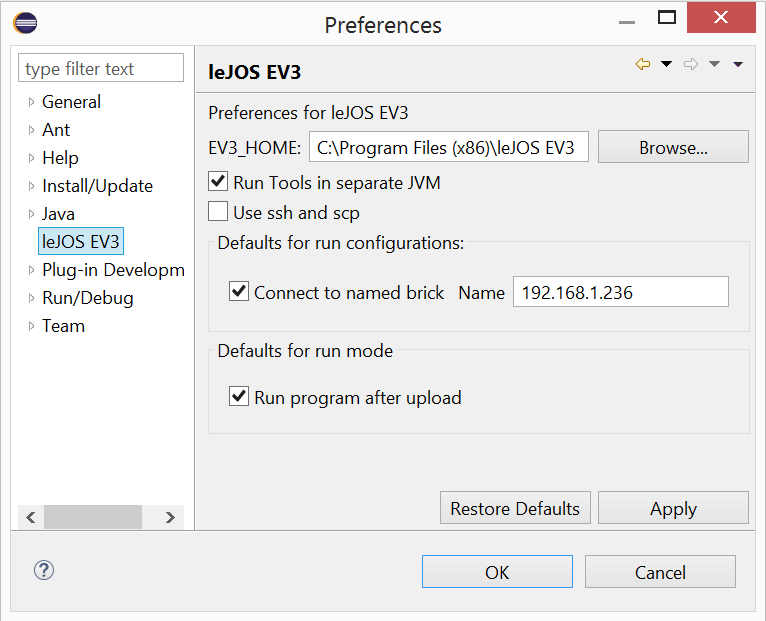
\includegraphics[scale=0.70]{img/Eclipse04.png}
	  	\caption{ }
		\end{figure}		
		
		\item After this is done any time you press the Run button, Eclipse will automatically upload your code to the brick and start it. Note, you will need to connect the brick to the computer via either USB, Bluetooth or WiFi for Eclipse to be able to upload to the robot. Hitting run with out an active connection will result in Eclipse creating the JAR file, then an error message will appear.
		\end{enumerate}	
  
   	\subsection{leJOS}
	Previously the leJOS Java Virtual Machine has been utilised within the SEP course in order to provide an interface for programming the NXT using the Java programming language. However as well as solid functions the leJOS NXT library had incomplete, untested and unimplemented methods, all of which handicapped SEP project development.\newline \newline
	
Given the incomplete nature of the previous library we were at first apprehensive, but given exposure to the leJOS EV3 library we are very satisfied with the progress that has occurred since the previous library.\\
An unexpected (yet highly desirable) addition was the inclusion of an RMI interface for the EV3 brick; this allows for simpler and streamlined code (compare the amount of code included in the following two figures) and also allows for a wider variety of system architectures.\\

A flaw of the original NXT kit was the uncertainty present at the beginning of the course as to whether all the sensor modules performed exactly as they were expected to; the new leJOS JVM soothes this uncertainty somewhat by providing a very thorough testing suite which can be launched from a freshly minted leJOS SD card.

	\begin{itemize}
		\item New features supported
		\item QWERTY on-screen-keyboard is a little unwieldy
		\item Longer boot time can be frustrating, but this is offset by the decreased need to reboot due to ease of uploading software from Eclipse and increased stability in LeJOS.
		\item 
	\end{itemize}
		\subsubsection{Java RMI}
	The EV3 version of the leJOS library allows EV3 devices to be accessed through a RMI (\textbf{R}emote \textbf{M}ethod \textbf{I}nvocation) interface; essentially this means that a PC (or other device) can call methods on the EV3 as if it were actually the EV3 itself!\\
An example of this is included in the figure below: \\
	\begin{figure}[H]
	  	\centering
	  	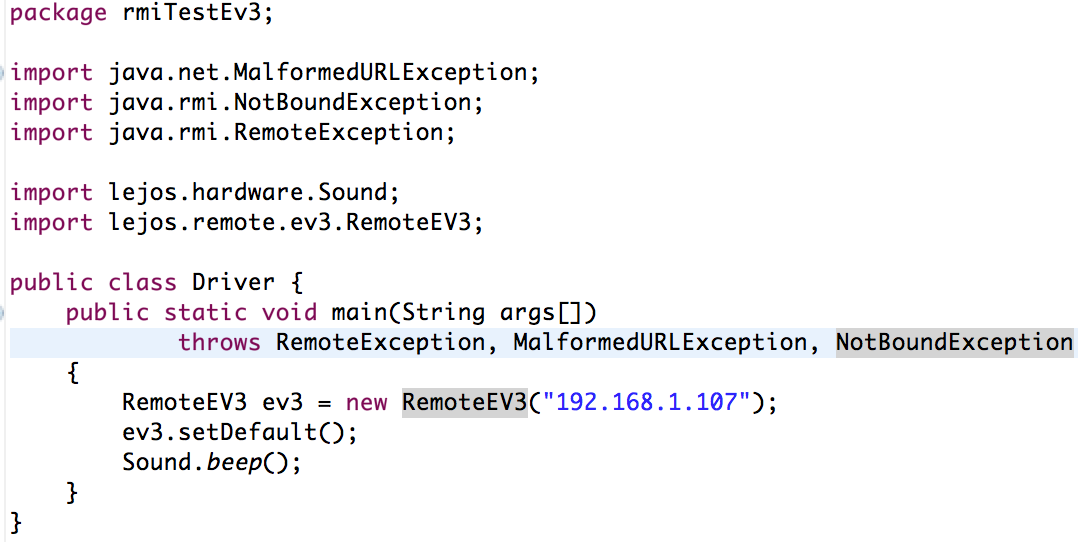
\includegraphics[scale=0.75]{img/EV3_RMI.png}
		\caption{A complete EV3 program which connects and sets the connected EV3 as the default device and triggers a Beep sound from the EV3s embedded speaker}
		\end{figure}	

This RMI interface works directly with leJOS; it's not required that there be a second program waiting on the EV3 device for method calls from the host computer.\\
If the programmer on the PC issues a command which conflicts with the current EV3 directive the new command will be queued to be enacted after the current command. For example if the EV3 has autonomously decided to move forward 10 centimetres and the programmer told the robot to move forward 3 centimetres the robot will move 3 centimeters \textbf{after} moving the previous 10 centimeters.

\begin{figure}[H]
	  	\centering
	  	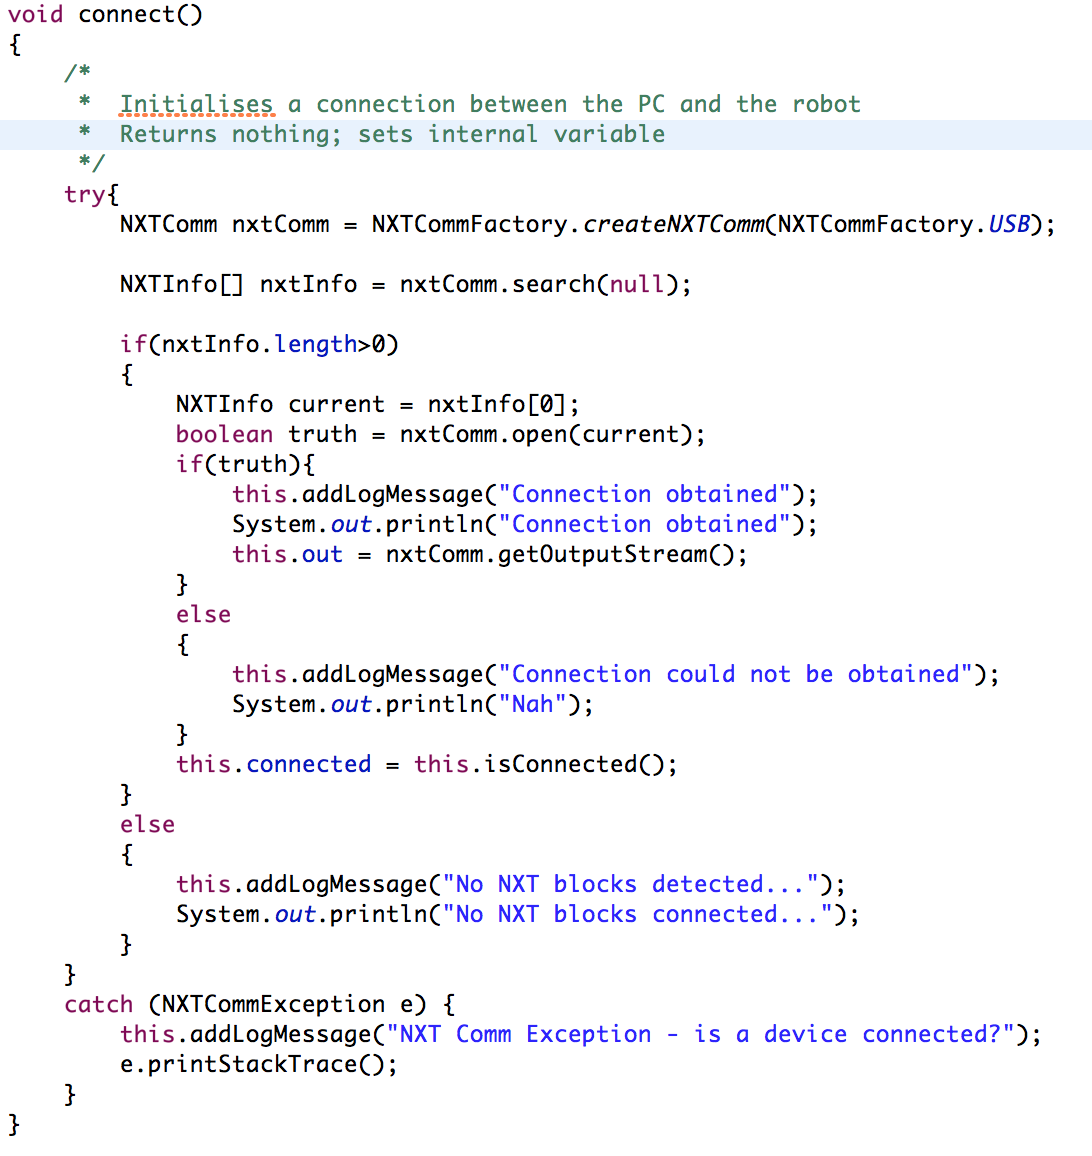
\includegraphics[scale=0.6]{img/EV3_NXT.png}
		\caption{A method inside a NXT program for obtaining a connection to the NXT device. Note the use of four custom classes \emph{just} for obtaining a connection.}
		\end{figure}	
	
	\begin{itemize}
		\item Explain what the RMI model involves
		\item Explain what this enables an EV3 programmer to do
		\item Give an example of a code block for this
	\end{itemize}
    Show examples, demonstrate different paradigms (e.g. setting one device as the 'default' block vs keeping a hold of several blocks)\\

	\subsubsection{Installation}
	See the following URL for installation details. \newline
	\url{http://sourceforge.net/p/lejos/wiki/Installing\%20leJOS/}
	\newline\newline
	A micro SD card is required for LeJOS to operate on the EV3 Brick. The older NXT Brick which lacked any expansion ports, had to replace the existing Lego software with LeJOS. The EV3 however can boot off the SD card directly, there by retaining the previous OS. However, this does mean that one micro SD card is required for each EV3 brick to operate LeJOS. \newline
	
	Creating the bootable SD card was simple on both Windows and OSX computers. There are a number of written and video tutorials available.
	
	\subsubsection{Operation}
Operation is simplistic; the hardest part is to insert a properly formatted SD card into the EV3 device and after which it will automatically launch after the initial firmware boots.
	
 	\section{Connectivity}
	A core feature of the NXT was its connectible nature; it could be programmed and controlled by a wide range of heterogeneous hardware and operating systems (including Windows, OSX and other Linux-based systems). \\
The EV3 has built upon this fundamental property by introducing a new connection method ( WiFi based connections) and by improving upon existing connections (for example by increasing the speed of USB connections enormously and by streamlining Bluetooth connectivity).
The change from the use of a proprietary operating system to a Unix-based one has also enabled greater connectivity; EV3 blocks can obtain and hold IP addresses which make them incredibly easy to address and connect to. Additionally the devices can also be SSHed directly to enabling very deep configurability of the OS and robot.
 	
	\subsection{WiFi}
   \begin{itemize}
    \item Requires the use of a WiFi dongle to activate WiFi capabilities. 
    \item Plug and play functionality (supports several mainstream chipsets)
    \item leJOS has a 'connection' menu item, IP address is clearly displayed
    \item Connect to a dedicated network just as you would any other device by using the leJOS WiFi tool to search for available networks, selecting the network then enter a password. If DHCP is setup on the network a new IP address will be given the the EV3 Brick so make sure your SSH tool or Eclipse has the latest IP address.
    \item Connections can be configured on the Micro SD image to avoid repeated configuration
    \item The EV3 appears to only have 2.4 GHz network support; the 5 GHz test network did not appear as a connectable option.
   \end{itemize}
 		\subsubsection{OSX}
			Tested, functional under OS X 10.9.\\
 		\subsubsection{Windows}
	 		Successfully tested under both Windows 7 and Windows 8.1.\\
	 	
 Once the Brick has successfully joined your network you can ping the IP address from any machine to check connection. If connection was successful, simply use the IP address to either SSH to the robot or enter the IP address into Eclipse for easy code uploading. (See step 12 of Section 3.1.1).
 			
 			
 	\subsection{Bluetooth}
  		\subsubsection{OSX}
		\begin{itemize}
			\item Still unable to simply connect via Bluetooth
			\item Technical forum posts show that other users' efforts are similarly problem affected
		\end{itemize}
  		\subsubsection{Windows}
		\begin{itemize}
			\item Easy Bluetooth connection using Windows 7
			\item Windows 8 connection slightly more tricky. Need to install the device as a Bluetooth device then go to "Devices and Printers", right click on the EV3 icon and select Connect As -> Access Point.
			\item Once connected, the EV3 brick has its own IP address. You can ping this to check connectivity.
			\item Can use SSH to copy files to and from the brick.
			\item Highly recommend Eclipse EV3 plugin as it simplifies the whole uploading process.
		\end{itemize}  		
  		
 	\subsection{USB}
    \begin{itemize}
      \item Device now has a USB host port (supports 3 levels of daisy chaining)
      \item Addition of standard USB port helps facilitate the use of a WiFi dongle and also allows for USB storage
      \item The new USB speed is a blistering 480 Mbit/s (compared to the NXTs 12 Mbit/s)

    \end{itemize}
 		\subsubsection{OSX}
Plug and play functionality; (once the Eclipse plugin was installed) I was able to push code to the block with a single button press.
 		\subsubsection{Windows}
	\textbf{TODO}

   	\section{Conclusion}
   		\subsection{Feasibility}
   		There is no doubt in our minds that the EV3 will be a great replacement for the NXT for the purpose of future projects. Every aspect of the NXT has been improved upon, ranging from the basic block design down to the advanced nature of the OS and modules. \\
   		
Increased sensitivity or functionality in all sensors greatly increases accuracy and stability of the robots functions. The changes in the API makes coding more intuitive with less code structural decisions that have to be 'worked around'.\\ 
   		
   		The improved API should drastically decrease the difficulty of the project. 
   		
   		
   		\subsection{Recommendations}
			Line following sensor combinations
			
			\begin{itemize}
			\item Single colour sensor as line and underground object detector. Gyroscope sensor for robot positioning feedback. Ultrasonic sensor for above ground object detector. Single bump sensor with a wide bar attached could be used as a collision detector to further improve on aboveground object detection.
			\item Single colour sensor as line and underground object detector. Gyroscope sensor for robot positioning feedback. Two bump sensors mounted on different parts of the robot for collision detection.
			
			\end{itemize}
			
			
   		\subsection{Additional project ideas}
   		These are ideas which may be suited for post-graduates. 
   		
   		\begin{itemize}
   		\item The EV3 brick comes with 4 motor ports, while 3 motors are supplied(2 large and one medium).  One idea could be to cannibalise some of the older NXT kits which contains 3 motors each and give the post-grads an extra NXT motor to accomplish an additional task such as picking up an object and placing it elsewhere or planting a flag on a designated area.
   		
   		\item The additional motor can be used to change orientation of some sensors to accomplish different tasks. Such as rotating the colour sensor from a vertical position during line following to a horizontal position when an above ground object is detected and it has to then detect the color of the above ground object and change it’s behaviour based on the detected colour.
   		
   		\item Both the light and colour sensor also has a decent Ambient light sensing mode. This can be utilised to perhaps have the robot find a source of light on the map or alternatively if the light source is made to flickers on and off in a programmed sequence, it can be used to transmit binary or Morse code for the Robot to maybe detect and interpret. 
   		
   		\item Given the nature of the leJOS operating system it may be possible to serve a robot control or data viewing interface over HTTP by using the EV3 as a web server.
   		
   		\item The gyroscope can be mounted on a motor arm which can change the orientation of the gyroscope to measure angle changes on multiple axis. This might be interesting if the robot is made to move over certain types of terrain. Or perhaps use the rate of change as a indicator of how quick the robot is turning and set either limits on the rate of turning to make sure the robot is slow and steady, or set goals for rate of turning to force robot in to quicker movements. 
   		\end{itemize}
   		
   		
		\subsection{Possible future project}
		A "Google car" project where the Robot has to stay within two lines on a map which simulates a lane on a road. This would be a good use of the light and colour sensors on each side of the robot or if one of these sensors is mounted on a sliding arm it could be used to detect variable size lanes. The ultrasonic sensor can be used to detect objects in front of robot to avoid collision or "park" within a certain distance to an object or even keep a minimum distance to another robot. \newline
		
		The robot needs to stop at intersections which can be denoted by either a series of lines perpendicular to the lane lines or possibly a particular coloured line at the intersection(yellow and red). The detected colour will trigger either a stop behaviour or a go behaviour. Once stopped perhaps a green colour card can be manually placed under the colour sensor to indicate it can now move forward to continue operations.\\
		It may be possible to automate intersections, however that may introduce a significant level of overhead (for example one solution is that the signals could be served by an auxilliary device connected to the same wifi network as the group of 'cars')  \newline 
		
		Additional requirements could be, the robot needs to perform tasks in a certain time constraint or speed. It may have to travel at a bounded speed to simulate speed limits. It might have to demonstrate different speeds depending on what speed zone it is currently in. Speed zones might be able to be represented by different coloured lanes.  \newline 
		
		Automatic parking behaviour can also be part of the project. If the robot is given a command it might have to look for a parking space, drive past it and then reverse parallel park in to it. This might involve scanning the parking area with the ultrasonic sensor to make sure the robot can fit in the space.  \newline 
		
		Multiple robots from different teams can even be placed on the map at the same time(assuming the map is of sufficient size) to make sure they behave correctly in the presence of moving objects.  \newline 
		
		Some of the requirements could be given to post-grads only. The test map would probably need to be A0 in size to allow a decent test area. 
		

  \newpage
  \section{Revision History}
  \begin{center}
  \begin{tabular}{ | l | l | l | p{6cm} |}
  \hline
  \textbf{\small Version} & \textbf{\small Date} & \textbf{\small Author} & \textbf{\small Description} \\ \hline
  \small 0.1 & \small 15 Dec 14 & \small Xiang Guo & \small Created Draft 1 \\ \hline
  \small 0.2 & \small 15 Dec 14 & \small Thomas McAtee & \small Added USB and connectivity section \\ \hline
  \small 0.3 & \small 16 Dec 14 & \small Thomas McAtee & \small Added more ToDos and bullet points \\ \hline
  \small 0.31 & \small 16 Dec 14 & \small Thomas McAtee & \small Added more to Connectivity and Software \\ \hline    
  \small 0.4 & \small 17 Dec 14 & \small Xiang Guo  & \small Added more detail to Hardware, Feasibility, Possible Future project and Additional project ideas. \\ \hline
  \small 0.5 & \small 18 Dec 14 & \small Thomas McAtee & \small Added more to section 3 and section 2 \\ \hline   
  \small 0.51 & \small 18 Dec 14 & \small Thomas McAtee & \small Merged RMI and leJOS sections in section 3 \\ \hline    
  \small 0.6 & \small 18 Dec 14 & \small Xiang Guo & \small Added Eclipse installation guide. \\ \hline
  \small 0.61 & \small 18 Dec 14 & \small Xiang Guo & \small Added Wifi for windows details and detailed revision history \\ \hline
  \end{tabular}
  \end{center}


\end{document}